\subtitle{Tag eins - Was ist Haskell} 
\date{24.03.2014}

\begin{frame}[plain]
\titlepage
\end{frame}

\section{Organisatorisches}
\begin{frame}
\frametitle{Organisatorisches}
\begin{block}{\vspace*{-3ex}}
	\begin{itemize}
	  \item Jeden Wochentag vom Mo, 24.03.2014 bis Fr, 28.03.2014 im Raum IZ 261.
	  \item 10:00 bis 16:00 Raumreservierung
	  \item 10:00 bis 11:30 theoretische Einführung in Haskell
	  \item 11:30 bis 12:30 Mittagspause
	  \item 12:30 bis ca. 15:30 praktische Übungen
	\end{itemize}
\end{block}
\end{frame}


\begin{frame}
\frametitle{Organisatorisches}
\begin{block}{\vspace*{-3ex}}
	\begin{itemize}
	  \item Theorie (jetzt)\\
	  		Umsetzung des Stoffs der Vorlesung in Haskell
	  \item Übungen (nachher)\\
	  		praktisches Arbeiten mit Haskell über den GHCi
	\end{itemize}
\end{block}
\end{frame}

\begin{frame}
\frametitle{Quellen}
\begin{block}{\vspace*{-3ex}}	
	\begin{itemize}
	  \item Algorithmieren und Programmieren\\ Vorlesung von Prof. Dr. Petra Hofstedt (BTU)
	  \item Moderne Funktionale Programmierung \\ Vorlesung von Prof. Dr. Petra Hofstedt (BTU)
	  \item Eine Einführung in die funktionale Programmierung mit Haskell \\ Übungsskript zu unserer Vorlesung
	  \item Haskell - Intensivkurs
	\end{itemize}
\end{block}
\end{frame}

\section{Das funktionale Paradigma}
\begin{frame}
\frametitle{Paradigmen}
\begin{block}{\vspace*{-3ex}}
\begin{itemize}
  \item Programmierparadigma\\
		generelle Sicht bei der Modellierung und Lösung eines Problems
  \item Klassische Unterscheidung
  \begin{itemize}
    \item Imperative Sprachen\\
    	 \textbf{"`Wie"'} findet die Lösung statt\\
    	 Folge von Anweisungen zur Problemlösung  
    \item Deklarative Sprachen \\
    	 \textbf{"`Was"'} ist die Lösung \\
    	 deklarative Beschreibung der Lösung bzw. des Problems
  \end{itemize}
\end{itemize}
\end{block}
\end{frame}

\begin{frame}
\frametitle{Paradigmen}
\begin{center}
\begin{tikzpicture}[>=stealth',shorten >=1pt,auto,node distance=2.5cm, xscale=2]
\node (Paradigmen)	{Paradigmen};
\node (imperativ) [below left of = Paradigmen]	{imperativ};
\node (prozedural) [below left of = imperativ]	{prozedural};
\node (oo) [below of = Paradigmen]	{objekt-orientiert};
\node (deklarativ) [below right of = Paradigmen]	{deklarativ};
\node (fl) [below left of = deklarativ]	{funktional-logisch};
\node (cl) [below right of = deklarativ]	{constraint-logisch};
\node (funktional) [below left of = fl]	{\textbf{funktional}};
\node (logisch) [right of = funktional]	{logisch};
\node (cb) [right of = logisch]	{constraint-basiert};

\path	(Paradigmen)	edge node { } (imperativ)
							edge node { } (deklarativ)
			(imperativ)		edge node { } (prozedural)
			(deklarativ)	edge node { } (fl)
							edge node { } (cl)
			(fl)			edge node { } (funktional)
							edge node { } (logisch)
			(cl)			edge node { } (logisch)
							edge node { } (cb);

\path[dashed]	(Paradigmen)	edge node { } (oo)
			(imperativ)		edge node { } (oo);		
\end{tikzpicture}
\end{center}
\end{frame}

\begin{frame}
\frametitle{Funktionale Paradigma}
\begin{block}{\vspace*{-3ex}}
\begin{itemize}
  \item Hohes Abstraktionsniveau \\ 
  Klare Darstellung der Programmiertechniken und Algorithmen,
d.h. Konzentration auf die Konzepte statt auf die Sprache.
  \item Klare, elegante und kompakte Programme \\ 
  kurze Entwicklungszeiten, lesbare Programme.
  \item Keine Seiteneffekte \\ 
  erleichtert Verstehen, Optimierung, Verifikation.
  \item Saubere theoretische Fundierung \\ 
  ermöglicht Verifikation und erleichtert formale Argumentation über Programme.
\end{itemize}
\end{block}
\end{frame}

\section{Haskell}
\begin{frame}
\frametitle{Haskell}
\begin{block}{\vspace*{-3ex}}
\begin{itemize}
  \item 1990 als Haskell 1.0 veröffentlicht
  \item Aktuelle Version Haskell 2010
  \item An Haskell 2014 (Preview) wird "`gearbeitet"'
\end{itemize}
\end{block}
\end{frame}

\begin{frame}[fragile]
\frametitle{Hello World} 
\begin{lstlisting}
module Main where
 
main :: IO ()
main = putStrLn "Hello, World!"
\end{lstlisting}
\pause
\begin{block}{Ausgabe}
\begin{center}
Hello, World!
\end{center}
\end{block}
\pause
\begin{center}
weiteres in den Übungen
\end{center}
\end{frame}

\begin{frame}
\frametitle{Haskell Compiler}
\begin{block}{\vspace*{-3ex}}
\begin{itemize}
  \item Hugs (Haskell User's Gofer System) \\ implementiert Haskell 98 \\ seit ca 6 Jahren nicht weiterentwickelt
  \item Yhc (York Haskell Compiler) \\ implementiert Haskell 98 \\ Projekt eingestellt
  \item GHC (Glasgow Haskell Compiler) \\ implementiert Haskell 98 / 2010 \\ weit verbreitster Haskell Compiler \\ 
  besitzt den GHCi als Haskell Interpreter \\ in den Übungen werden wir hauptsächlich mit dem Interpreter arbeiten
\end{itemize}
\end{block}
\end{frame}

\begin{frame}
\frametitle{Glasgow Haskell Compiler}
\begin{block}{\vspace*{-3ex}}
\begin{itemize}
  \item Original Prototyp '89 in LML (Lazy ML) 
  \item Bei der Entwicklung von Haskell in Haskell neu geschrieben ('89)
  \item Nur kleine Teile in C bzw. C-- (C verwandte Sprache zur Nutzung als Zwischencode)
  \item Erweitert den Haskell Standard um noch nicht standardisierte Erweiterungen
  \item Plattform und Architektur unabhängig
\end{itemize}
\end{block}
\end{frame}

\begin{frame}
\frametitle{Laufzeitumgebung}
\begin{block}{\vspace*{-3ex}}
\begin{itemize}
  \item Wenn das Programm in Maschinencode übersetzt wurde, wird keine externe Laufzeitumgebung benötigt (nativer Code)\\
  		die "`Laufzeitumgebung"' wird mit in das Programm gepackt
  \item Bei Benutzung des Interpreters wird dieser als Laufzeitumgebung verwendet.
\end{itemize}
\end{block}
\end{frame}

\begin{frame}
\frametitle{Interne Funktionsweise}
\begin{block}{\vspace*{-3ex}}
\begin{itemize}
  \item Erzeugung von Zwischencode "`C--"'
  \item C-- ist wie C-Code jedoch "`etwas"' anders
  \item Dieser Code wird optimiert und weiter compiliert
  \item "`-fasm"' erzeugt Maschinencode (Standard)
  \item "`-fvia-C"' erzeugt C-Code aus C--\\
  		seit Version 7.0 nicht mehr unterstützt
  \item "`-fllvm"' nutzt den LLVM als Backend-Compiler
\end{itemize}
\end{block}
\end{frame}

\begin{frame}
\frametitle{Interne Funktionsweise}
\begin{figure}
\centering
\includegraphics*[scale=0.4]{images/HscPipe2_1}
\caption{Compiler Teil 1 \copyright haskell.org}
\end{figure}
\end{frame}


\begin{frame}
\frametitle{Interne Funktionsweise}
\begin{figure}
\centering
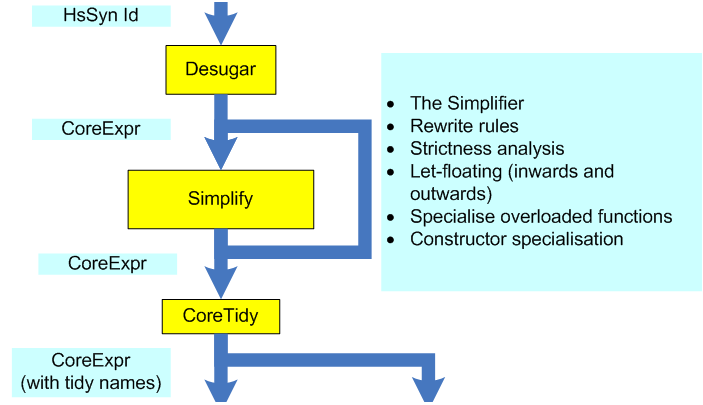
\includegraphics[scale=0.4]{images/HscPipe2_2.png}
\caption{Compiler Teil 2 \copyright haskell.org}
\end{figure}
\end{frame}

\begin{frame}
\frametitle{Interne Funktionsweise}
\begin{figure}
\centering
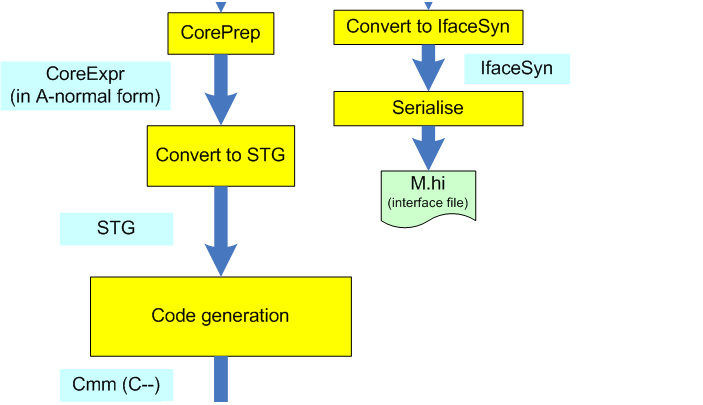
\includegraphics[scale=0.4]{images/HscPipe2_3.png}
\caption{Compiler Teil 3 \copyright haskell.org}
\end{figure}
\end{frame}

\begin{frame}
\frametitle{Interne Funktionsweise}
\begin{figure}
\centering
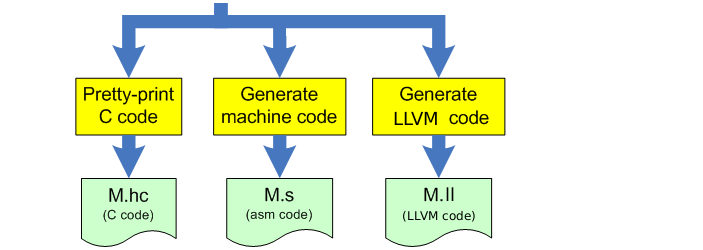
\includegraphics[scale=0.4]{images/HscPipe2_4.png}
\caption{Compiler Teil 4 \copyright haskell.org}
\end{figure}
\end{frame}

\section{Semantische Grundbegriffe}

\subsection{Namen und Attribute}
\begin{frame}
\frametitle{Namen und Attribute}
\begin{block}{\vspace*{-3ex}}
\begin{itemize}
  \item Alle endlichen ASCII-Strings außer:
  \\ \lstinline|case|, \lstinline|class|, \lstinline|data|, \lstinline|default|, \lstinline|deriving|, \lstinline|do|, \lstinline|else|, \lstinline|if|, \lstinline|import|, \lstinline|in|, \lstinline|infix|, \lstinline|infixl|, \lstinline|infixr|, \lstinline|instance|, \lstinline|let|, \lstinline|module|, \lstinline|newtype|, \lstinline|of|, \lstinline|then|, \lstinline|type|, \lstinline|where|
  \item Bezeichner sind case-sensitiv. (\lstinline|pLus| $\neq$ \lstinline|plus|) 
  \item \lstinline|_| (Unterstrich) ist der Platzhalter
  \item Module beginnen mit einem Großbuchstaben
  \item Funktionen mit einem Kleinbuchstaben
\end{itemize}
\end{block}
\end{frame}

\subsection{Variablen und Konstanten}
\begin{frame}
\frametitle{Variablen}
\begin{block}{\vspace*{-3ex}}
\begin{itemize}
  \item Globale Variablen existieren nicht
  \item Lokale Variablen existieren nur in Funktionen als Teilergebnis
\end{itemize}
\end{block}
\end{frame}

\begin{frame}
\frametitle{Konstanten}
\begin{block}{\vspace*{-3ex}}
%\begin{itemize}
%  \item Konstanten sind Funktionen ohne Parameter
%\end{itemize}
Konstanten sind Funktionen ohne Parameter
\end{block}
\end{frame}

\subsection{Ausdrücke}
\begin{frame}
\frametitle{Ausdrücke}
\begin{block}{\vspace*{-3ex}}
elementare Ausdrücke bzw. Grundterme setzten sich zusammen aus:
\begin{itemize}
  \item Konstanten wie z.B. Zahlen (\lstinline|10|, \lstinline|9.8|), Zeichen (\lstinline|'a'|, \lstinline|'Z'|), \ldots
  \item Andere Funktionen \lstinline|sin|, \lstinline|+|, \lstinline|*|, \ldots
\end{itemize}
\end{block}
\begin{alertblock}{Infixnotation}
Funktionszeichen: \lstinline|3 + 4| $\equiv$ \lstinline|(+) 3 4|\\
Funktionsname: \lstinline|mod 100 4| $\equiv$ \lstinline|100 `mod` 4|
\end{alertblock}
\end{frame}

\begin{frame}
\frametitle{Ausdrücke}
\begin{block}{\vspace*{-3ex}}
\begin{itemize}
  \item Elementare Ausdrücke mit Variablen sind Ausdrücke bzw. Terme
  \item Durch einen "`Vorspann"' wie $\ x$ wird die Variable $x$ mit der $\lambda$-Notation "`gebunden"'
  \item $\lambda a \to \lambda b \to a + b$ ist ein $\lambda$-Ausdruck
  \item $\lambda$ ist kein ASCII Zeichen, deswegen wird "`\textbackslash"' verwendet 
\end{itemize}
\end{block}
\end{frame}

\begin{frame}[fragile]
\frametitle{Ausdrücke} 
\begin{exampleblock}{Elementarer Ausdruck}
\lstinline|plus = 10 + 30|
\end{exampleblock}
\begin{exampleblock}{Ausdruck}
\lstinline|plus' a b = a + b|
\end{exampleblock}
\begin{exampleblock}{Lambda ($\lambda$)-Ausdruck}
\lstinline|plus'' =  \\a -> \\b -> a + b|\\
Morgen kommt mehr zum Thema $\lambda$-Ausdrücke
\end{exampleblock}
\end{frame}

\subsection{Funktionen}
\begin{frame}
\frametitle{Deklaration von Funktionen}
\begin{block}{\vspace*{-3ex}}
\begin{itemize}
  \item Funktion $f$ ist ein Tripel $(D_f, W_f, R_f)$
  \item $D_f$ Definitionsmenge
  \item $W_f$ Wertemenge
  \item $R_f \subseteq D_f \times W_f$
  \item $R_f$ muss \textbf{rechtseindeutig} sein d.h. es gibt keine zwei Paare $(a,b1) \in R_f$ und $(a,b_2) \in R_f$ mit $b_1 \neq b_2$
  \item Somit gilt, eine Funktion $f$ bildet den Argumentwert $x$ in den Resultatwert $y$ ab 
\end{itemize}
\end{block}
\end{frame}

\begin{frame}
\frametitle{Deklaration von Funktionen}
\only<1>{
\vspace*{-1ex}
\begin{exampleblock}{Konstante}
\begin{center}
\scalebox{0.6}{\begin{tikzpicture}[
      nonterminal/.style={
         rectangle,
         minimum size=5.0mm,
         very thick,
         draw=blue!50!black!50,
         top color=white,
         bottom color=blue!50!black!20,
         font=\itshape\scriptsize,
         %text height=1.5ex,
         %text depth=.25ex
      },
      terminal/.style={
         rounded rectangle,
         minimum size=5.0mm,
         very thick,draw=black!50,
         top color=white,bottom color=black!20,
         font=\ttfamily\scriptsize,
         %text height=1.5ex,
         %text depth=.25ex
      },
      skip loop/.style={
         to path={-- ++(0,#1) -| (\tikztotarget)}
      },
      point/.style={coordinate},>=stealth',thick,draw=black!50,
      tip/.style={->,shorten >=0.007pt},every join/.style={rounded corners},
      hv path/.style={to path={-| (\tikztotarget)}},
      vh path/.style={to path={|- (\tikztotarget)}},
      %text height=1.5ex,text depth=.25ex
    ]
    \matrix[column sep=5.0mm, row sep=3.0mm] {
 &  & \node (n13) [nonterminal] {Bezeichner}; & \node (n14) [terminal] {::}; & \node (n15) [nonterminal] {Typ Erg}; & \node (n16) [terminal] {LF}; &  & \\
\node (n21) [circle, draw, inner sep=0pt, minimum size=0.75ex] {}; & \node (n22) [point] {}; &  &  &  &  & \node (n27) [point] {}; & \node (n28) [point] {};\\
 &  & \node (n33) [point] {}; &  &  &  &  & \\
 &  &  &  &  &  &  & \\
 &  &  &  & \node (n55) [nonterminal] {Wert}; &  &  & \\
\node (n61) [point] {}; & \node (n62) [nonterminal] {Bezeichner}; & \node (n63) [terminal] {=}; & \node (n64) [point] {}; &  & \node (n66) [point] {}; & \node (n67) [terminal] {LF}; & \node (n68) [circle, draw, inner sep=0pt, minimum size=0.75ex] {};\\
 &  &  &  & \node (n75) [nonterminal] {Ausdruck}; &  &  & \\
    };
  { [start chain]
       \chainin (n21);
       \chainin (n22)    [join];
  }
  { [start chain]
       \chainin (n22);
       \chainin (n13)    [join=by {vh path,tip}];
  }
  { [start chain]
       \chainin (n13);
       \chainin (n14)    [join=by tip];
  }
  { [start chain]
       \chainin (n14);
       \chainin (n15)    [join=by tip];
  }
  { [start chain]
       \chainin (n15);
       \chainin (n16)    [join=by tip];
  }
  { [start chain]
       \chainin (n16);
       \chainin (n27)    [join=by {hv path}];
  }
  { [start chain]
       \chainin (n22);
       \chainin (n33)    [join=by {vh path}];
  }
  { [start chain]
       \chainin (n33);
       \chainin (n27)    [join=by {hv path}];
  }
  { [start chain]
       \chainin (n27);
       \chainin (n28)    [join=by tip];
  }
  { [start chain]
       \chainin (n61);
       \chainin (n62)    [join=by tip];
  }
  { [start chain]
       \chainin (n62);
       \chainin (n63)    [join=by tip];
  }
  { [start chain]
       \chainin (n63);
       \chainin (n64)    [join];
  }
  { [start chain]
       \chainin (n64);
       \chainin (n55)    [join=by {vh path,tip}];
  }
  { [start chain]
       \chainin (n55);
       \chainin (n66)    [join=by {hv path}];
  }
  { [start chain]
       \chainin (n64);
       \chainin (n75)    [join=by {vh path,tip}];
  }
  { [start chain]
       \chainin (n75);
       \chainin (n66)    [join=by {hv path}];
  }
  { [start chain]
       \chainin (n66);
       \chainin (n67)    [join=by tip];
  }
  { [start chain]
       \chainin (n67);
       \chainin (n68)    [join=by tip];
  }
\end{tikzpicture}
}
\end{center}
\end{exampleblock}}
\only<2>{
\vspace*{-1ex}
\begin{exampleblock}{Funktion}
\begin{center}
\scalebox{0.5}{\begin{tikzpicture}[
      nonterminal/.style={
         rectangle,
         minimum size=5.0mm,
         very thick,
         draw=blue!50!black!50,
         top color=white,
         bottom color=blue!50!black!20,
         font=\itshape\scriptsize,
         %text height=1.5ex,
         %text depth=.25ex
      },
      terminal/.style={
         rounded rectangle,
         minimum size=5.0mm,
         very thick,draw=black!50,
         top color=white,bottom color=black!20,
         font=\ttfamily\scriptsize,
         %text height=1.5ex,
         %text depth=.25ex
      },
      skip loop/.style={
         to path={-- ++(0,#1) -| (\tikztotarget)}
      },
      point/.style={coordinate},>=stealth',thick,draw=black!50,
      tip/.style={->,shorten >=0.007pt},every join/.style={rounded corners},
      hv path/.style={to path={-| (\tikztotarget)}},
      vh path/.style={to path={|- (\tikztotarget)}},
      %text height=1.5ex,text depth=.25ex
    ]
    \matrix[column sep=5.0mm, row sep=3.0mm] {
 &  &  &  &  & \node (n16) [point] {}; &  &  &  &  &  &  & \\
 &  & \node (n23) [nonterminal] {Bezeichner}; & \node (n24) [terminal] {::}; & \node (n25) [point] {}; & \node (n26) [nonterminal] {Typ Para}; & \node (n27) [terminal] {->}; & \node (n28) [point] {}; & \node (n29) [nonterminal] {Typ Erg}; & \node (n210) [terminal] {LF}; &  &  & \\
\node (n31) [circle, draw, inner sep=0pt, minimum size=0.75ex] {}; & \node (n32) [point] {}; &  &  &  &  &  &  &  &  & \node (n311) [point] {}; & \node (n312) [point] {}; & \\
 &  & \node (n43) [point] {}; &  &  &  &  &  &  &  &  &  & \\
 &  &  &  &  &  &  &  &  &  &  &  & \\
 &  &  &  &  &  & \node (n67) [point] {}; &  &  &  &  &  & \\
 &  &  &  & \node (n75) [point] {}; &  &  &  & \node (n79) [nonterminal] {Wert}; &  &  &  & \\
\node (n81) [point] {}; & \node (n82) [point] {}; & \node (n83) [nonterminal] {Bezeichner}; & \node (n84) [point] {}; & \node (n85) [nonterminal] {Bezeichner Para}; & \node (n86) [point] {}; & \node (n87) [terminal] {=}; & \node (n88) [point] {}; &  & \node (n810) [point] {}; & \node (n811) [terminal] {LF}; & \node (n812) [point] {}; & \node (n813) [circle, draw, inner sep=0pt, minimum size=0.75ex] {};\\
 &  &  &  &  &  &  &  & \node (n99) [nonterminal] {Ausdruck}; &  &  &  & \\
    };
  { [start chain]
       \chainin (n31);
       \chainin (n32)    [join];
  }
  { [start chain]
       \chainin (n32);
       \chainin (n23)    [join=by {vh path,tip}];
  }
  { [start chain]
       \chainin (n23);
       \chainin (n24)    [join=by tip];
  }
  { [start chain]
       \chainin (n24);
       \chainin (n25)    [join];
  }
  { [start chain]
       \chainin (n25);
       \chainin (n26)    [join=by tip];
  }
  { [start chain]
       \chainin (n26);
       \chainin (n27)    [join=by tip];
  }
  { [start chain]
       \chainin (n27);
       \chainin (n28)    [join];
  }
  { [start chain]
       \chainin (n28);
       \chainin (n29)    [join=by tip];
  }
  { [start chain]
       \chainin (n29);
       \chainin (n210)    [join=by tip];
  }
  { [start chain]
       \chainin (n210);
       \chainin (n311)    [join=by {hv path}];
  }
  { [start chain]
       \chainin (n32);
       \chainin (n43)    [join=by {vh path}];
  }
  { [start chain]
       \chainin (n43);
       \chainin (n311)    [join=by {hv path}];
  }
  { [start chain]
       \chainin (n311);
       \chainin (n312)    [join=by tip];
  }
  { [start chain]
       \chainin (n81);
       \chainin (n82)    [join];
  }
  { [start chain]
       \chainin (n82);
       \chainin (n83)    [join=by tip];
  }
  { [start chain]
       \chainin (n83);
       \chainin (n84)    [join];
  }
  { [start chain]
       \chainin (n84);
       \chainin (n85)    [join=by tip];
  }
  { [start chain]
       \chainin (n85);
       \chainin (n86)    [join];
  }
  { [start chain]
       \chainin (n86);
       \chainin (n87)    [join=by tip];
  }
  { [start chain]
       \chainin (n87);
       \chainin (n88)    [join];
  }
  { [start chain]
       \chainin (n88);
       \chainin (n79)    [join=by {vh path,tip}];
  }
  { [start chain]
       \chainin (n79);
       \chainin (n810)    [join=by {hv path}];
  }
  { [start chain]
       \chainin (n88);
       \chainin (n99)    [join=by {vh path,tip}];
  }
  { [start chain]
       \chainin (n99);
       \chainin (n810)    [join=by {hv path}];
  }
  { [start chain]
       \chainin (n810);
       \chainin (n811)    [join=by tip];
  }
  { [start chain]
       \chainin (n811);
       \chainin (n812)    [join];
  }
  { [start chain]
       \chainin (n812);
       \chainin (n813)    [join=by tip];
  }
  { [start chain]
       \chainin (n28);
       \chainin (n16)    [join=by vh path];
       \chainin (n25)    [join=by {hv path,tip}];
  }
  { [start chain]
       \chainin (n86);
       \chainin (n75)    [join=by vh path];
       \chainin (n84)    [join=by {hv path,tip}];
  }
  { [start chain]
       \chainin (n812);
       \chainin (n67)    [join=by vh path];
       \chainin (n82)    [join=by {hv path,tip}];
  }
\end{tikzpicture}
}
\end{center}
\end{exampleblock}}
\only<3>{\begin{exampleblock}{Allgemein}
\begin{center}
\scalebox{0.6}{\begin{tikzpicture}[
      nonterminal/.style={
         rectangle,
         minimum size=5.0mm,
         very thick,
         draw=blue!50!black!50,
         top color=white,
         bottom color=blue!50!black!20,
         font=\itshape\scriptsize,
         %text height=1.5ex,
         %text depth=.25ex
      },
      terminal/.style={
         rounded rectangle,
         minimum size=5.0mm,
         very thick,draw=black!50,
         top color=white,bottom color=black!20,
         font=\ttfamily\scriptsize,
         %text height=1.5ex,
         %text depth=.25ex
      },
      skip loop/.style={
         to path={-- ++(0,#1) -| (\tikztotarget)}
      },
      point/.style={coordinate},>=stealth',thick,draw=black!50,
      tip/.style={->,shorten >=0.007pt},every join/.style={rounded corners},
      hv path/.style={to path={-| (\tikztotarget)}},
      vh path/.style={to path={|- (\tikztotarget)}},
      %text height=1.5ex,text depth=.25ex
    ]
    \matrix[column sep=5.0mm, row sep=3.0mm] {
 &  &  &  &  & \node (n16) [terminal] {->}; & \node (n17) [nonterminal] {Typ Para}; &  &  &  &  &  & \\
 &  & \node (n23) [nonterminal] {Bezeichner}; & \node (n24) [terminal] {::}; & \node (n25) [point] {}; &  &  & \node (n28) [point] {}; & \node (n29) [nonterminal] {Typ Erg}; & \node (n210) [terminal] {LF}; &  &  & \\
\node (n31) [circle, draw, inner sep=0pt, minimum size=0.75ex] {}; & \node (n32) [point] {}; &  &  &  &  &  &  &  &  & \node (n311) [point] {}; & \node (n312) [point] {}; & \\
 &  & \node (n43) [point] {}; &  &  &  &  &  &  &  &  &  & \\
 &  &  &  &  &  &  &  &  &  &  &  & \\
 &  &  &  &  &  & \node (n67) [point] {}; &  &  &  &  &  & \\
 &  &  &  & \node (n75) [nonterminal] {Bezeichner Para}; &  &  &  & \node (n79) [nonterminal] {Wert}; &  &  &  & \\
\node (n81) [point] {}; & \node (n82) [point] {}; & \node (n83) [nonterminal] {Bezeichner}; & \node (n84) [point] {}; &  & \node (n86) [point] {}; & \node (n87) [terminal] {=}; & \node (n88) [point] {}; &  & \node (n810) [point] {}; & \node (n811) [terminal] {LF}; & \node (n812) [point] {}; & \node (n813) [circle, draw, inner sep=0pt, minimum size=0.75ex] {};\\
 &  &  &  &  &  &  &  & \node (n99) [nonterminal] {Ausdruck}; &  &  &  & \\
    };
  { [start chain]
       \chainin (n31);
       \chainin (n32)    [join];
  }
  { [start chain]
       \chainin (n32);
       \chainin (n23)    [join=by {vh path,tip}];
  }
  { [start chain]
       \chainin (n23);
       \chainin (n24)    [join=by tip];
  }
  { [start chain]
       \chainin (n24);
       \chainin (n25)    [join];
  }
  { [start chain]
       \chainin (n25);
       \chainin (n28)    [join];
  }
  { [start chain]
       \chainin (n17);
       \chainin (n16)    [join=by tip];
  }
  { [start chain]
       \chainin (n28);
       \chainin (n17)    [join=by {vh path,tip}];
  }
  { [start chain]
       \chainin (n16);
       \chainin (n25)    [join=by {hv path,tip}];
  }
  { [start chain]
       \chainin (n28);
       \chainin (n29)    [join=by tip];
  }
  { [start chain]
       \chainin (n29);
       \chainin (n210)    [join=by tip];
  }
  { [start chain]
       \chainin (n210);
       \chainin (n311)    [join=by {hv path}];
  }
  { [start chain]
       \chainin (n32);
       \chainin (n43)    [join=by {vh path}];
  }
  { [start chain]
       \chainin (n43);
       \chainin (n311)    [join=by {hv path}];
  }
  { [start chain]
       \chainin (n311);
       \chainin (n312)    [join=by tip];
  }
  { [start chain]
       \chainin (n81);
       \chainin (n82)    [join];
  }
  { [start chain]
       \chainin (n82);
       \chainin (n83)    [join=by tip];
  }
  { [start chain]
       \chainin (n83);
       \chainin (n84)    [join];
  }
  { [start chain]
       \chainin (n84);
       \chainin (n86)    [join];
  }
  { [start chain]
       \chainin (n86);
       \chainin (n75)    [join=by {vh path,tip}];
  }
  { [start chain]
       \chainin (n75);
       \chainin (n84)    [join=by {hv path,tip}];
  }
  { [start chain]
       \chainin (n86);
       \chainin (n87)    [join=by tip];
  }
  { [start chain]
       \chainin (n87);
       \chainin (n88)    [join];
  }
  { [start chain]
       \chainin (n88);
       \chainin (n79)    [join=by {vh path,tip}];
  }
  { [start chain]
       \chainin (n79);
       \chainin (n810)    [join=by {hv path}];
  }
  { [start chain]
       \chainin (n88);
       \chainin (n99)    [join=by {vh path,tip}];
  }
  { [start chain]
       \chainin (n99);
       \chainin (n810)    [join=by {hv path}];
  }
  { [start chain]
       \chainin (n810);
       \chainin (n811)    [join=by tip];
  }
  { [start chain]
       \chainin (n811);
       \chainin (n812)    [join];
  }
  { [start chain]
       \chainin (n812);
       \chainin (n813)    [join=by tip];
  }
  { [start chain]
       \chainin (n812);
       \chainin (n67)    [join=by vh path];
       \chainin (n82)    [join=by {hv path,tip}];
  }
\end{tikzpicture}
}
\end{center}
\end{exampleblock}}
\only<1-2>{\vspace*{-3ex}
\begin{block}{\vspace*{-3ex}}
\begin{itemize} 
  \item Funktionsköpfe sind optional, jedoch empfohlen
  \item Funktionsnamen beginnen mit Kleinbuchstaben
  \item Parameter von Funktionen beginnen mit Kleinbuchstaben
\end{itemize}
\end{block}}
\end{frame}

\begin{frame}[fragile]
\frametitle{Deklaration von Funktionen} 
\begin{exampleblock}{Konstante}
\begin{lstlisting}
eins :: Int
eins  = 1
\end{lstlisting}
\end{exampleblock}
\end{frame}

\begin{frame}[fragile]
\frametitle{Deklaration von Funktionen} 
\begin{exampleblock}{Konstante}
\begin{lstlisting}
eins :: Int
eins  = 1
\end{lstlisting}
\end{exampleblock}
\begin{exampleblock}{Unäre Funktion}
\begin{lstlisting}
successor :: Int -> Int
successor      a  = a + 1
\end{lstlisting}
\end{exampleblock}
\end{frame}

\begin{frame}[fragile]
\frametitle{Deklaration von Funktionen} 
\vspace*{-2.5ex}
\begin{exampleblock}{Konstante}
\begin{lstlisting}
eins :: Int
eins  = 1
\end{lstlisting}
\end{exampleblock}
\vspace*{-3ex}
\begin{exampleblock}{Unäre Funktion}
\begin{lstlisting}
successor :: Int -> Int
successor      a  = a + 1
\end{lstlisting}
\end{exampleblock}
\vspace*{-3ex}
\begin{exampleblock}{Binäre Funktion}
\begin{lstlisting}
nimmDenZweiten :: Int -> Int -> Int
nimmDenZweiten    _      b    = b
\end{lstlisting}
\end{exampleblock}
\end{frame}

\begin{frame}
\frametitle{Funktionen vs. Operatoren}
\begin{block}{\vspace*{-3ex}}
\begin{itemize}
  \item Funktionen besitzen einen Namen aus Buchstaben
  \item Operatoren besitzen einen Namen aus Zeichen
  \item Funktionen binden stärker als Operatoren (Standard)
  \item Operatoren werden wie Funktionen deklariert
\end{itemize}
\end{block}
\end{frame}

\subsection{Blöcke}
\begin{frame}
\frametitle{Der where Block}
\vspace*{-3ex}
\begin{block}{\vspace*{-3ex}}
\begin{itemize}
  \item Zur nachträglichen Definition von internen Hilfsfunktionen (Teilfunktionen)
  %\item {}<ober Funktion> \dots = <Hilfsfunktion> + <Ausdruck> \\ \textbf{where} \\ <Hilfsfunktion> \dots = \dots
  \item Verschachtelung erlaubt
  \item Definiert für die ganze Funktion
  \item "`Funktionsköpfe"' erlaubt
\end{itemize}
\end{block}
\only<2>{
\vspace*{-2ex}
	\begin{exampleblock}{\vspace*{-3ex}}
	\begin{center}
	\vspace*{-2ex}
	\scalebox{0.45}{\begin{tikzpicture}[
      nonterminal/.style={
         rectangle,
         minimum size=5.0mm,
         very thick,
         draw=blue!50!black!50,
         top color=white,
         bottom color=blue!50!black!20,
         font=\itshape\scriptsize,
         %text height=1.5ex,
         %text depth=.25ex
      },
      terminal/.style={
         rounded rectangle,
         minimum size=5.0mm,
         very thick,draw=black!50,
         top color=white,bottom color=black!20,
         font=\ttfamily\scriptsize,
         %text height=1.5ex,
         %text depth=.25ex
      },
      skip loop/.style={
         to path={-- ++(0,#1) -| (\tikztotarget)}
      },
      point/.style={coordinate},>=stealth',thick,draw=black!50,
      tip/.style={->,shorten >=0.007pt},every join/.style={rounded corners},
      hv path/.style={to path={-| (\tikztotarget)}},
      vh path/.style={to path={|- (\tikztotarget)}},
      %text height=1.5ex,text depth=.25ex
    ]
    \matrix[column sep=5.0mm, row sep=3.0mm] {
 &  &  &  &  &  &  &  & \node (n19) [point] {}; &  &  &  &  &  &  &  &  &  &  & \\
 &  &  & \node (n24) [point] {}; &  &  &  &  & \node (n29) [nonterminal] {Ausdruck}; &  &  &  &  &  &  &  &  &  &  & \\
\node (n31) [circle, draw, inner sep=0pt, minimum size=0.75ex] {}; & \node (n32) [nonterminal] {Funktion}; & \node (n33) [point] {}; & \node (n34) [nonterminal] {Parameter}; & \node (n35) [point] {}; & \node (n36) [terminal] {=}; & \node (n37) [point] {}; & \node (n38) [point] {}; &  & \node (n310) [point] {}; & \node (n311) [point] {}; & \node (n312) [terminal] {LF}; & \node (n313) [point] {}; &  &  &  &  &  &  & \\
 &  &  &  &  &  &  &  & \node (n49) [nonterminal] {Hilfsfunktion}; &  &  &  &  &  &  &  &  &  &  & \\
 &  &  &  &  &  &  &  &  &  &  &  &  &  &  &  &  &  &  & \\
 &  &  &  &  &  &  &  &  & \node (n610) [point] {}; &  &  &  &  &  &  &  &  &  & \\
 &  &  &  &  &  &  &  &  &  &  & \node (n712) [point] {}; &  &  &  &  &  &  &  & \\
 &  &  &  &  &  &  &  &  &  &  &  &  & \node (n814) [point] {}; &  &  &  &  &  & \\
 &  &  &  &  &  &  &  & \node (n99) [point] {}; &  &  &  &  & \node (n914) [nonterminal] {Ausdruck}; &  &  &  &  &  & \\
\node (n101) [point] {}; & \node (n102) [point] {}; & \node (n103) [terminal] {Tab}; & \node (n104) [terminal] {where}; & \node (n105) [terminal] {LF}; & \node (n106) [point] {}; & \node (n107) [nonterminal] {Hilfsfunktion}; & \node (n108) [point] {}; & \node (n109) [nonterminal] {Parameter}; & \node (n1010) [point] {}; & \node (n1011) [terminal] {=}; & \node (n1012) [point] {}; & \node (n1013) [point] {}; &  & \node (n1015) [point] {}; & \node (n1016) [point] {}; & \node (n1017) [terminal] {LF}; & \node (n1018) [point] {}; & \node (n1019) [point] {}; & \node (n1020) [circle, draw, inner sep=0pt, minimum size=0.75ex] {};\\
 &  &  &  &  &  &  &  &  &  &  &  &  & \node (n1114) [nonterminal] {Hilfsfunktion}; &  &  &  &  &  & \\
    };
  { [start chain]
       \chainin (n31);
       \chainin (n32)    [join=by tip];
  }
  { [start chain]
       \chainin (n32);
       \chainin (n33)    [join];
  }
  { [start chain]
       \chainin (n33);
       \chainin (n34)    [join=by tip];
  }
  { [start chain]
       \chainin (n34);
       \chainin (n35)    [join];
  }
  { [start chain]
       \chainin (n35);
       \chainin (n36)    [join=by tip];
  }
  { [start chain]
       \chainin (n36);
       \chainin (n37)    [join];
  }
  { [start chain]
       \chainin (n37);
       \chainin (n38)    [join];
  }
  { [start chain]
       \chainin (n38);
       \chainin (n29)    [join=by {vh path,tip}];
  }
  { [start chain]
       \chainin (n29);
       \chainin (n310)    [join=by {hv path}];
  }
  { [start chain]
       \chainin (n38);
       \chainin (n49)    [join=by {vh path,tip}];
  }
  { [start chain]
       \chainin (n49);
       \chainin (n310)    [join=by {hv path}];
  }
  { [start chain]
       \chainin (n310);
       \chainin (n311)    [join];
  }
  { [start chain]
       \chainin (n311);
       \chainin (n312)    [join=by tip];
  }
  { [start chain]
       \chainin (n312);
       \chainin (n313)    [join=by tip];
  }
  { [start chain]
       \chainin (n101);
       \chainin (n102)    [join];
  }
  { [start chain]
       \chainin (n102);
       \chainin (n103)    [join=by tip];
  }
  { [start chain]
       \chainin (n103);
       \chainin (n104)    [join=by tip];
  }
  { [start chain]
       \chainin (n104);
       \chainin (n105)    [join=by tip];
  }
  { [start chain]
       \chainin (n105);
       \chainin (n106)    [join];
  }
  { [start chain]
       \chainin (n106);
       \chainin (n107)    [join=by tip];
  }
  { [start chain]
       \chainin (n107);
       \chainin (n108)    [join];
  }
  { [start chain]
       \chainin (n108);
       \chainin (n109)    [join=by tip];
  }
  { [start chain]
       \chainin (n109);
       \chainin (n1010)    [join];
  }
  { [start chain]
       \chainin (n1010);
       \chainin (n1011)    [join=by tip];
  }
  { [start chain]
       \chainin (n1011);
       \chainin (n1012)    [join];
  }
  { [start chain]
       \chainin (n1012);
       \chainin (n1013)    [join];
  }
  { [start chain]
       \chainin (n1013);
       \chainin (n914)    [join=by {vh path,tip}];
  }
  { [start chain]
       \chainin (n914);
       \chainin (n1015)    [join=by {hv path}];
  }
  { [start chain]
       \chainin (n1013);
       \chainin (n1114)    [join=by {vh path,tip}];
  }
  { [start chain]
       \chainin (n1114);
       \chainin (n1015)    [join=by {hv path}];
  }
  { [start chain]
       \chainin (n1015);
       \chainin (n1016)    [join];
  }
  { [start chain]
       \chainin (n1016);
       \chainin (n1017)    [join=by tip];
  }
  { [start chain]
       \chainin (n1017);
       \chainin (n1018)    [join];
  }
  { [start chain]
       \chainin (n1018);
       \chainin (n1019)    [join];
  }
  { [start chain]
       \chainin (n1019);
       \chainin (n1020)    [join=by tip];
  }
  { [start chain]
       \chainin (n35);
       \chainin (n24)    [join=by vh path];
       \chainin (n33)    [join=by {hv path,tip}];
  }
  { [start chain]
       \chainin (n311);
       \chainin (n19)    [join=by vh path];
       \chainin (n37)    [join=by {hv path,tip}];
  }
  { [start chain]
       \chainin (n1010);
       \chainin (n99)    [join=by vh path];
       \chainin (n108)    [join=by {hv path,tip}];
  }
  { [start chain]
       \chainin (n1016);
       \chainin (n814)    [join=by vh path];
       \chainin (n1012)    [join=by {hv path,tip}];
  }
  { [start chain]
       \chainin (n1018);
       \chainin (n712)    [join=by vh path];
       \chainin (n106)    [join=by {hv path,tip}];
  }
  { [start chain]
       \chainin (n1019);
       \chainin (n610)    [join=by vh path];
       \chainin (n102)    [join=by {hv path,tip}];
  }
\end{tikzpicture}
}
	\end{center}
	\end{exampleblock}
}
\end{frame}

\begin{frame}[fragile]
\frametitle{Der where Block}
\begin{lstlisting}
dec a = inc a - 2
    where	
        inc a = a + 1
\end{lstlisting}
\begin{exampleblock}{\vspace*{-3ex}}
\begin{center}
\vspace*{-1ex}
\scalebox{0.45}{\begin{tikzpicture}[
      nonterminal/.style={
         rectangle,
         minimum size=5.0mm,
         very thick,
         draw=blue!50!black!50,
         top color=white,
         bottom color=blue!50!black!20,
         font=\itshape\scriptsize,
         %text height=1.5ex,
         %text depth=.25ex
      },
      terminal/.style={
         rounded rectangle,
         minimum size=5.0mm,
         very thick,draw=black!50,
         top color=white,bottom color=black!20,
         font=\ttfamily\scriptsize,
         %text height=1.5ex,
         %text depth=.25ex
      },
      skip loop/.style={
         to path={-- ++(0,#1) -| (\tikztotarget)}
      },
      point/.style={coordinate},>=stealth',thick,draw=black!50,
      tip/.style={->,shorten >=0.007pt},every join/.style={rounded corners},
      hv path/.style={to path={-| (\tikztotarget)}},
      vh path/.style={to path={|- (\tikztotarget)}},
      %text height=1.5ex,text depth=.25ex
    ]
    \matrix[column sep=5.0mm, row sep=3.0mm] {
 &  &  &  &  &  &  &  & \node (n19) [point] {}; &  &  &  &  &  &  &  &  &  &  & \\
 &  &  & \node (n24) [point] {}; &  &  &  &  & \node (n29) [nonterminal] {Ausdruck}; &  &  &  &  &  &  &  &  &  &  & \\
\node (n31) [circle, draw, inner sep=0pt, minimum size=0.75ex] {}; & \node (n32) [nonterminal] {Funktion}; & \node (n33) [point] {}; & \node (n34) [nonterminal] {Parameter}; & \node (n35) [point] {}; & \node (n36) [terminal] {=}; & \node (n37) [point] {}; & \node (n38) [point] {}; &  & \node (n310) [point] {}; & \node (n311) [point] {}; & \node (n312) [terminal] {LF}; & \node (n313) [point] {}; &  &  &  &  &  &  & \\
 &  &  &  &  &  &  &  & \node (n49) [nonterminal] {Hilfsfunktion}; &  &  &  &  &  &  &  &  &  &  & \\
 &  &  &  &  &  &  &  &  &  &  &  &  &  &  &  &  &  &  & \\
 &  &  &  &  &  &  &  &  & \node (n610) [point] {}; &  &  &  &  &  &  &  &  &  & \\
 &  &  &  &  &  &  &  &  &  &  & \node (n712) [point] {}; &  &  &  &  &  &  &  & \\
 &  &  &  &  &  &  &  &  &  &  &  &  & \node (n814) [point] {}; &  &  &  &  &  & \\
 &  &  &  &  &  &  &  & \node (n99) [point] {}; &  &  &  &  & \node (n914) [nonterminal] {Ausdruck}; &  &  &  &  &  & \\
\node (n101) [point] {}; & \node (n102) [point] {}; & \node (n103) [terminal] {Tab}; & \node (n104) [terminal] {where}; & \node (n105) [terminal] {LF}; & \node (n106) [point] {}; & \node (n107) [nonterminal] {Hilfsfunktion}; & \node (n108) [point] {}; & \node (n109) [nonterminal] {Parameter}; & \node (n1010) [point] {}; & \node (n1011) [terminal] {=}; & \node (n1012) [point] {}; & \node (n1013) [point] {}; &  & \node (n1015) [point] {}; & \node (n1016) [point] {}; & \node (n1017) [terminal] {LF}; & \node (n1018) [point] {}; & \node (n1019) [point] {}; & \node (n1020) [circle, draw, inner sep=0pt, minimum size=0.75ex] {};\\
 &  &  &  &  &  &  &  &  &  &  &  &  & \node (n1114) [nonterminal] {Hilfsfunktion}; &  &  &  &  &  & \\
    };
  { [start chain]
       \chainin (n31);
       \chainin (n32)    [join=by tip];
  }
  { [start chain]
       \chainin (n32);
       \chainin (n33)    [join];
  }
  { [start chain]
       \chainin (n33);
       \chainin (n34)    [join=by tip];
  }
  { [start chain]
       \chainin (n34);
       \chainin (n35)    [join];
  }
  { [start chain]
       \chainin (n35);
       \chainin (n36)    [join=by tip];
  }
  { [start chain]
       \chainin (n36);
       \chainin (n37)    [join];
  }
  { [start chain]
       \chainin (n37);
       \chainin (n38)    [join];
  }
  { [start chain]
       \chainin (n38);
       \chainin (n29)    [join=by {vh path,tip}];
  }
  { [start chain]
       \chainin (n29);
       \chainin (n310)    [join=by {hv path}];
  }
  { [start chain]
       \chainin (n38);
       \chainin (n49)    [join=by {vh path,tip}];
  }
  { [start chain]
       \chainin (n49);
       \chainin (n310)    [join=by {hv path}];
  }
  { [start chain]
       \chainin (n310);
       \chainin (n311)    [join];
  }
  { [start chain]
       \chainin (n311);
       \chainin (n312)    [join=by tip];
  }
  { [start chain]
       \chainin (n312);
       \chainin (n313)    [join=by tip];
  }
  { [start chain]
       \chainin (n101);
       \chainin (n102)    [join];
  }
  { [start chain]
       \chainin (n102);
       \chainin (n103)    [join=by tip];
  }
  { [start chain]
       \chainin (n103);
       \chainin (n104)    [join=by tip];
  }
  { [start chain]
       \chainin (n104);
       \chainin (n105)    [join=by tip];
  }
  { [start chain]
       \chainin (n105);
       \chainin (n106)    [join];
  }
  { [start chain]
       \chainin (n106);
       \chainin (n107)    [join=by tip];
  }
  { [start chain]
       \chainin (n107);
       \chainin (n108)    [join];
  }
  { [start chain]
       \chainin (n108);
       \chainin (n109)    [join=by tip];
  }
  { [start chain]
       \chainin (n109);
       \chainin (n1010)    [join];
  }
  { [start chain]
       \chainin (n1010);
       \chainin (n1011)    [join=by tip];
  }
  { [start chain]
       \chainin (n1011);
       \chainin (n1012)    [join];
  }
  { [start chain]
       \chainin (n1012);
       \chainin (n1013)    [join];
  }
  { [start chain]
       \chainin (n1013);
       \chainin (n914)    [join=by {vh path,tip}];
  }
  { [start chain]
       \chainin (n914);
       \chainin (n1015)    [join=by {hv path}];
  }
  { [start chain]
       \chainin (n1013);
       \chainin (n1114)    [join=by {vh path,tip}];
  }
  { [start chain]
       \chainin (n1114);
       \chainin (n1015)    [join=by {hv path}];
  }
  { [start chain]
       \chainin (n1015);
       \chainin (n1016)    [join];
  }
  { [start chain]
       \chainin (n1016);
       \chainin (n1017)    [join=by tip];
  }
  { [start chain]
       \chainin (n1017);
       \chainin (n1018)    [join];
  }
  { [start chain]
       \chainin (n1018);
       \chainin (n1019)    [join];
  }
  { [start chain]
       \chainin (n1019);
       \chainin (n1020)    [join=by tip];
  }
  { [start chain]
       \chainin (n35);
       \chainin (n24)    [join=by vh path];
       \chainin (n33)    [join=by {hv path,tip}];
  }
  { [start chain]
       \chainin (n311);
       \chainin (n19)    [join=by vh path];
       \chainin (n37)    [join=by {hv path,tip}];
  }
  { [start chain]
       \chainin (n1010);
       \chainin (n99)    [join=by vh path];
       \chainin (n108)    [join=by {hv path,tip}];
  }
  { [start chain]
       \chainin (n1016);
       \chainin (n814)    [join=by vh path];
       \chainin (n1012)    [join=by {hv path,tip}];
  }
  { [start chain]
       \chainin (n1018);
       \chainin (n712)    [join=by vh path];
       \chainin (n106)    [join=by {hv path,tip}];
  }
  { [start chain]
       \chainin (n1019);
       \chainin (n610)    [join=by vh path];
       \chainin (n102)    [join=by {hv path,tip}];
  }
\end{tikzpicture}
}
\end{center}
\end{exampleblock}
\end{frame}

\begin{frame}[fragile]
\frametitle{Der where Block}
\begin{lstlisting}
f :: Int -> Int 
f   a   = x a `div` 3
    where x b = y b * 2
        where y b = a + b + 1 
\end{lstlisting}
\only<1>{
\begin{exampleblock}{\vspace*{-3ex}}
\begin{center}
\vspace*{-1ex}
\scalebox{0.45}{\begin{tikzpicture}[
      nonterminal/.style={
         rectangle,
         minimum size=5.0mm,
         very thick,
         draw=blue!50!black!50,
         top color=white,
         bottom color=blue!50!black!20,
         font=\itshape\scriptsize,
         %text height=1.5ex,
         %text depth=.25ex
      },
      terminal/.style={
         rounded rectangle,
         minimum size=5.0mm,
         very thick,draw=black!50,
         top color=white,bottom color=black!20,
         font=\ttfamily\scriptsize,
         %text height=1.5ex,
         %text depth=.25ex
      },
      skip loop/.style={
         to path={-- ++(0,#1) -| (\tikztotarget)}
      },
      point/.style={coordinate},>=stealth',thick,draw=black!50,
      tip/.style={->,shorten >=0.007pt},every join/.style={rounded corners},
      hv path/.style={to path={-| (\tikztotarget)}},
      vh path/.style={to path={|- (\tikztotarget)}},
      %text height=1.5ex,text depth=.25ex
    ]
    \matrix[column sep=5.0mm, row sep=3.0mm] {
 &  &  &  &  &  &  &  & \node (n19) [point] {}; &  &  &  &  &  &  &  &  &  &  & \\
 &  &  & \node (n24) [point] {}; &  &  &  &  & \node (n29) [nonterminal] {Ausdruck}; &  &  &  &  &  &  &  &  &  &  & \\
\node (n31) [circle, draw, inner sep=0pt, minimum size=0.75ex] {}; & \node (n32) [nonterminal] {Funktion}; & \node (n33) [point] {}; & \node (n34) [nonterminal] {Parameter}; & \node (n35) [point] {}; & \node (n36) [terminal] {=}; & \node (n37) [point] {}; & \node (n38) [point] {}; &  & \node (n310) [point] {}; & \node (n311) [point] {}; & \node (n312) [terminal] {LF}; & \node (n313) [point] {}; &  &  &  &  &  &  & \\
 &  &  &  &  &  &  &  & \node (n49) [nonterminal] {Hilfsfunktion}; &  &  &  &  &  &  &  &  &  &  & \\
 &  &  &  &  &  &  &  &  &  &  &  &  &  &  &  &  &  &  & \\
 &  &  &  &  &  &  &  &  & \node (n610) [point] {}; &  &  &  &  &  &  &  &  &  & \\
 &  &  &  &  &  &  &  &  &  &  & \node (n712) [point] {}; &  &  &  &  &  &  &  & \\
 &  &  &  &  &  &  &  &  &  &  &  &  & \node (n814) [point] {}; &  &  &  &  &  & \\
 &  &  &  &  &  &  &  & \node (n99) [point] {}; &  &  &  &  & \node (n914) [nonterminal] {Ausdruck}; &  &  &  &  &  & \\
\node (n101) [point] {}; & \node (n102) [point] {}; & \node (n103) [terminal] {Tab}; & \node (n104) [terminal] {where}; & \node (n105) [terminal] {LF}; & \node (n106) [point] {}; & \node (n107) [nonterminal] {Hilfsfunktion}; & \node (n108) [point] {}; & \node (n109) [nonterminal] {Parameter}; & \node (n1010) [point] {}; & \node (n1011) [terminal] {=}; & \node (n1012) [point] {}; & \node (n1013) [point] {}; &  & \node (n1015) [point] {}; & \node (n1016) [point] {}; & \node (n1017) [terminal] {LF}; & \node (n1018) [point] {}; & \node (n1019) [point] {}; & \node (n1020) [circle, draw, inner sep=0pt, minimum size=0.75ex] {};\\
 &  &  &  &  &  &  &  &  &  &  &  &  & \node (n1114) [nonterminal] {Hilfsfunktion}; &  &  &  &  &  & \\
    };
  { [start chain]
       \chainin (n31);
       \chainin (n32)    [join=by tip];
  }
  { [start chain]
       \chainin (n32);
       \chainin (n33)    [join];
  }
  { [start chain]
       \chainin (n33);
       \chainin (n34)    [join=by tip];
  }
  { [start chain]
       \chainin (n34);
       \chainin (n35)    [join];
  }
  { [start chain]
       \chainin (n35);
       \chainin (n36)    [join=by tip];
  }
  { [start chain]
       \chainin (n36);
       \chainin (n37)    [join];
  }
  { [start chain]
       \chainin (n37);
       \chainin (n38)    [join];
  }
  { [start chain]
       \chainin (n38);
       \chainin (n29)    [join=by {vh path,tip}];
  }
  { [start chain]
       \chainin (n29);
       \chainin (n310)    [join=by {hv path}];
  }
  { [start chain]
       \chainin (n38);
       \chainin (n49)    [join=by {vh path,tip}];
  }
  { [start chain]
       \chainin (n49);
       \chainin (n310)    [join=by {hv path}];
  }
  { [start chain]
       \chainin (n310);
       \chainin (n311)    [join];
  }
  { [start chain]
       \chainin (n311);
       \chainin (n312)    [join=by tip];
  }
  { [start chain]
       \chainin (n312);
       \chainin (n313)    [join=by tip];
  }
  { [start chain]
       \chainin (n101);
       \chainin (n102)    [join];
  }
  { [start chain]
       \chainin (n102);
       \chainin (n103)    [join=by tip];
  }
  { [start chain]
       \chainin (n103);
       \chainin (n104)    [join=by tip];
  }
  { [start chain]
       \chainin (n104);
       \chainin (n105)    [join=by tip];
  }
  { [start chain]
       \chainin (n105);
       \chainin (n106)    [join];
  }
  { [start chain]
       \chainin (n106);
       \chainin (n107)    [join=by tip];
  }
  { [start chain]
       \chainin (n107);
       \chainin (n108)    [join];
  }
  { [start chain]
       \chainin (n108);
       \chainin (n109)    [join=by tip];
  }
  { [start chain]
       \chainin (n109);
       \chainin (n1010)    [join];
  }
  { [start chain]
       \chainin (n1010);
       \chainin (n1011)    [join=by tip];
  }
  { [start chain]
       \chainin (n1011);
       \chainin (n1012)    [join];
  }
  { [start chain]
       \chainin (n1012);
       \chainin (n1013)    [join];
  }
  { [start chain]
       \chainin (n1013);
       \chainin (n914)    [join=by {vh path,tip}];
  }
  { [start chain]
       \chainin (n914);
       \chainin (n1015)    [join=by {hv path}];
  }
  { [start chain]
       \chainin (n1013);
       \chainin (n1114)    [join=by {vh path,tip}];
  }
  { [start chain]
       \chainin (n1114);
       \chainin (n1015)    [join=by {hv path}];
  }
  { [start chain]
       \chainin (n1015);
       \chainin (n1016)    [join];
  }
  { [start chain]
       \chainin (n1016);
       \chainin (n1017)    [join=by tip];
  }
  { [start chain]
       \chainin (n1017);
       \chainin (n1018)    [join];
  }
  { [start chain]
       \chainin (n1018);
       \chainin (n1019)    [join];
  }
  { [start chain]
       \chainin (n1019);
       \chainin (n1020)    [join=by tip];
  }
  { [start chain]
       \chainin (n35);
       \chainin (n24)    [join=by vh path];
       \chainin (n33)    [join=by {hv path,tip}];
  }
  { [start chain]
       \chainin (n311);
       \chainin (n19)    [join=by vh path];
       \chainin (n37)    [join=by {hv path,tip}];
  }
  { [start chain]
       \chainin (n1010);
       \chainin (n99)    [join=by vh path];
       \chainin (n108)    [join=by {hv path,tip}];
  }
  { [start chain]
       \chainin (n1016);
       \chainin (n814)    [join=by vh path];
       \chainin (n1012)    [join=by {hv path,tip}];
  }
  { [start chain]
       \chainin (n1018);
       \chainin (n712)    [join=by vh path];
       \chainin (n106)    [join=by {hv path,tip}];
  }
  { [start chain]
       \chainin (n1019);
       \chainin (n610)    [join=by vh path];
       \chainin (n102)    [join=by {hv path,tip}];
  }
\end{tikzpicture}
}
\end{center}
\end{exampleblock}}
\only<2-3>{
\begin{exampleblock}{Aufruf}
\lstinline|f 4|
\end{exampleblock}}
\only<3>{
\begin{exampleblock}{Ausgabe}
\lstinline|6|
\end{exampleblock}}
\end{frame}

\begin{frame}
\frametitle{Der let-in Block}
\only<1>{\begin{block}{\vspace*{-3ex}}
\begin{itemize}
  \item Zur vorherigen Definition von internen Hilfsfunktionen (Teilfunktionen)
  %\item {[} <ober Funktion> \dots = {]} \\ \textbf{let} <Hilfsfunktion> \dots = \dots \\ {[}\textbf{in} 
  % <Hilfsfunktion> + <Ausdruck> {]}
  \item Kann auch zur Definition von Funktionen im Interpreter verwendet werden  
  \item Verschachtelung erlaubt
  \item Definiert für den Funktionsabschnitt 
\end{itemize}
\end{block}}
\only<2>{\begin{exampleblock}{\vspace*{-3ex}}
\begin{center}
\scalebox{0.45}{\begin{tikzpicture}[
      nonterminal/.style={
         rectangle,
         minimum size=5.0mm,
         very thick,
         draw=blue!50!black!50,
         top color=white,
         bottom color=blue!50!black!20,
         font=\itshape\scriptsize,
         %text height=1.5ex,
         %text depth=.25ex
      },
      terminal/.style={
         rounded rectangle,
         minimum size=5.0mm,
         very thick,draw=black!50,
         top color=white,bottom color=black!20,
         font=\ttfamily\scriptsize,
         %text height=1.5ex,
         %text depth=.25ex
      },
      skip loop/.style={
         to path={-- ++(0,#1) -| (\tikztotarget)}
      },
      point/.style={coordinate},>=stealth',thick,draw=black!50,
      tip/.style={->,shorten >=0.007pt},every join/.style={rounded corners},
      hv path/.style={to path={-| (\tikztotarget)}},
      vh path/.style={to path={|- (\tikztotarget)}},
      %text height=1.5ex,text depth=.25ex
    ]
    \matrix[column sep=5.0mm, row sep=3.0mm] {
 &  &  & \node (n14) [point] {}; &  &  &  &  &  &  &  &  &  &  &  &  &  & \\
\node (n21) [circle, draw, inner sep=0pt, minimum size=0.75ex] {}; & \node (n22) [nonterminal] {Funktion}; & \node (n23) [point] {}; & \node (n24) [nonterminal] {Parameter}; & \node (n25) [point] {}; & \node (n26) [terminal] {=}; & \node (n27) [terminal] {LF}; & \node (n28) [point] {}; &  &  &  &  &  &  &  &  &  & \\
 &  &  &  &  &  &  &  &  &  &  &  &  &  &  &  &  & \\
 &  &  &  &  &  &  &  &  &  & \node (n411) [point] {}; &  &  &  &  &  &  & \\
 &  &  &  &  &  &  &  &  &  &  &  & \node (n513) [point] {}; &  &  &  &  & \\
 &  &  &  &  &  &  & \node (n68) [point] {}; &  &  &  &  & \node (n613) [nonterminal] {Ausdruck}; &  &  &  &  & \\
\node (n71) [point] {}; & \node (n72) [terminal] {Tab}; & \node (n73) [terminal] {let}; & \node (n74) [terminal] {LF}; & \node (n75) [point] {}; & \node (n76) [nonterminal] {Hilfsfunktion}; & \node (n77) [point] {}; & \node (n78) [nonterminal] {Parameter}; & \node (n79) [point] {}; & \node (n710) [terminal] {=}; & \node (n711) [point] {}; & \node (n712) [point] {}; &  & \node (n714) [point] {}; & \node (n715) [point] {}; & \node (n716) [terminal] {LF}; & \node (n717) [point] {}; & \node (n718) [point] {};\\
 &  &  &  &  &  &  &  &  &  &  &  & \node (n813) [nonterminal] {TiefereHilfsfunktion}; &  &  &  &  & \\
 &  &  &  &  &  &  &  &  &  &  &  &  &  &  &  &  & \\
 &  &  & \node (n104) [nonterminal] {Ausdruck}; &  &  &  &  &  &  &  &  &  &  &  &  &  & \\
\node (n111) [point] {}; & \node (n112) [terminal] {in}; & \node (n113) [point] {}; &  & \node (n115) [point] {}; & \node (n116) [circle, draw, inner sep=0pt, minimum size=0.75ex] {}; &  &  &  &  &  &  &  &  &  &  &  & \\
 &  &  & \node (n124) [nonterminal] {Hilfsfunktion}; &  &  &  &  &  &  &  &  &  &  &  &  &  & \\
    };
  { [start chain]
       \chainin (n21);
       \chainin (n22)    [join=by tip];
  }
  { [start chain]
       \chainin (n22);
       \chainin (n23)    [join];
  }
  { [start chain]
       \chainin (n23);
       \chainin (n24)    [join=by tip];
  }
  { [start chain]
       \chainin (n24);
       \chainin (n25)    [join];
  }
  { [start chain]
       \chainin (n25);
       \chainin (n26)    [join=by tip];
  }
  { [start chain]
       \chainin (n26);
       \chainin (n27)    [join=by tip];
  }
  { [start chain]
       \chainin (n27);
       \chainin (n28)    [join=by tip];
  }
  { [start chain]
       \chainin (n71);
       \chainin (n72)    [join=by tip];
  }
  { [start chain]
       \chainin (n72);
       \chainin (n73)    [join=by tip];
  }
  { [start chain]
       \chainin (n73);
       \chainin (n74)    [join=by tip];
  }
  { [start chain]
       \chainin (n74);
       \chainin (n75)    [join];
  }
  { [start chain]
       \chainin (n75);
       \chainin (n76)    [join=by tip];
  }
  { [start chain]
       \chainin (n76);
       \chainin (n77)    [join];
  }
  { [start chain]
       \chainin (n77);
       \chainin (n78)    [join=by tip];
  }
  { [start chain]
       \chainin (n78);
       \chainin (n79)    [join];
  }
  { [start chain]
       \chainin (n79);
       \chainin (n710)    [join=by tip];
  }
  { [start chain]
       \chainin (n710);
       \chainin (n711)    [join];
  }
  { [start chain]
       \chainin (n711);
       \chainin (n712)    [join];
  }
  { [start chain]
       \chainin (n712);
       \chainin (n613)    [join=by {vh path,tip}];
  }
  { [start chain]
       \chainin (n613);
       \chainin (n714)    [join=by {hv path}];
  }
  { [start chain]
       \chainin (n712);
       \chainin (n813)    [join=by {vh path,tip}];
  }
  { [start chain]
       \chainin (n813);
       \chainin (n714)    [join=by {hv path}];
  }
  { [start chain]
       \chainin (n714);
       \chainin (n715)    [join];
  }
  { [start chain]
       \chainin (n715);
       \chainin (n716)    [join=by tip];
  }
  { [start chain]
       \chainin (n716);
       \chainin (n717)    [join];
  }
  { [start chain]
       \chainin (n717);
       \chainin (n718)    [join=by tip];
  }
  { [start chain]
       \chainin (n111);
       \chainin (n112)    [join=by tip];
  }
  { [start chain]
       \chainin (n112);
       \chainin (n113)    [join];
  }
  { [start chain]
       \chainin (n113);
       \chainin (n104)    [join=by {vh path,tip}];
  }
  { [start chain]
       \chainin (n104);
       \chainin (n115)    [join=by {hv path}];
  }
  { [start chain]
       \chainin (n113);
       \chainin (n124)    [join=by {vh path,tip}];
  }
  { [start chain]
       \chainin (n124);
       \chainin (n115)    [join=by {hv path}];
  }
  { [start chain]
       \chainin (n115);
       \chainin (n116)    [join=by tip];
  }
  { [start chain]
       \chainin (n25);
       \chainin (n14)    [join=by vh path];
       \chainin (n23)    [join=by {hv path,tip}];
  }
  { [start chain]
       \chainin (n79);
       \chainin (n68)    [join=by vh path];
       \chainin (n77)    [join=by {hv path,tip}];
  }
  { [start chain]
       \chainin (n715);
       \chainin (n513)    [join=by vh path];
       \chainin (n711)    [join=by {hv path,tip}];
  }
  { [start chain]
       \chainin (n717);
       \chainin (n411)    [join=by vh path];
       \chainin (n75)    [join=by {hv path,tip}];
  }
\end{tikzpicture}
}\\
Blöcke mit let-in können verschachtelt sein\\
Bei mehr als einer Hilfsfunktion, muss nach dem \lstinline|let| ein Zeilenumbruch erfolgen.
\end{center}
\end{exampleblock}}
\end{frame}

\begin{frame}[fragile]
\frametitle{Der let-in Block}
\begin{lstlisting}
dec a = 
  let               
      inc1 a = a + 1
      inc2 a = a + 2
  in  inc1 a - inc2 0
\end{lstlisting}
\only<1>{\begin{exampleblock}{Zur Definition von Funktionen direkt im GHCi}
\lstinline|let {plus :: Int -> Int -> Int; plus a b = a + b}|
\end{exampleblock}}
\only<2-3>{
\begin{exampleblock}{Aufruf}
\lstinline|dec 42|
\end{exampleblock}}
\only<3>{
\begin{exampleblock}{Ausgabe}
\lstinline|41|
\end{exampleblock}}
\end{frame}

\begin{frame}[fragile]
\frametitle{Der let-in Block}
\begin{lstlisting}
outer a = 
    let mid b = 
        let inner c = c + 1
        in inner b + 2
    in mid a + 3	
\end{lstlisting}
\only<1-2>{
\begin{exampleblock}{Aufruf}
\lstinline|outer 42|
\end{exampleblock}}
\only<2>{
\begin{exampleblock}{Ausgabe}
\lstinline|48|
\end{exampleblock}}
\end{frame}

\section{Einfache Datentypen}
\begin{frame}
\frametitle{Einfache Datentypen}
\begin{block}{\vspace*{-3ex}}
\begin{itemize}
  \item \lstinline|Bool|
  \item \lstinline|Int|
  \item \lstinline|Integer|
  \item \lstinline|Float|
  \item \lstinline|Double|
  \item \lstinline|Char|
\end{itemize}
\end{block}
\end{frame}
\subsection{Warheitswerte}
\begin{frame}
\frametitle{\lstinline|Bool|}
\begin{block}{\vspace*{-3ex}}
\begin{itemize}
  \item Einfacher Wahrheitswert
  \item \lstinline|True| oder \lstinline|False|
  \item \lstinline|not| $\equiv$ Verneinung
  \item \lstinline|&&| (binär), \lstinline|and| (Liste) $\equiv$ und
  \item \lstinline!||! (binär), \lstinline|or| (Liste) $\equiv$ oder
  \item \lstinline|==| $\equiv$ gleich
  \item \lstinline|/=| $\equiv$ ungleich
\end{itemize}
\end{block}
\end{frame}

\begin{frame}[fragile]
\frametitle{\lstinline|Bool|} 
\begin{lstlisting}
myAnd :: Bool -> Bool -> Bool
myAnd True True  = True
myAnd _    _     = False

myOr :: Bool -> Bool -> Bool
myOr False False = False
myOr _     _     = True
\end{lstlisting}
\end{frame}
\subsection{Ganzzahlen}
\begin{frame}
\frametitle{\lstinline|Int|}
\begin{block}{\vspace*{-3ex}}
\begin{itemize}
  \item 32 Bit Ganzzahl (Architektur abhängig)
  \item Min = $-2^{31} = -2147483648$
  \item Max = $2^{31} - 1 = 2147483647$
  \item Zirkulär $(2^{31} - 1) + 1 = -2^{31}$ 
\end{itemize}
\end{block}
\begin{alertblock}{Achtung}
\lstinline|Int| ist nicht gleich \lstinline|Integer|!
\end{alertblock}
\end{frame}

\begin{frame}
\frametitle{\lstinline|Integer|}
\begin{block}{\vspace*{-3ex}}
\begin{itemize}
  \item Unbegrenzte Ganzzahl (RAM Größe ist die "`Begrenzung"')
  \item Bei unendlich Arbeitsspeicher wirklich unbegrenzt
\end{itemize}
\end{block}
\end{frame}

\begin{frame}[fragile]
\frametitle{\lstinline|Int| vs \lstinline|Integer|} 
\begin{lstlisting}
plus :: Int -> Int -> Int
plus a b = a + b
\end{lstlisting}
\only<1-2>{
\begin{exampleblock}{Aufruf}
\lstinline|plus 2147483647 1|
\end{exampleblock}}
\only<2>{
\begin{exampleblock}{Ausgabe}
\lstinline|-2147483648|
\end{exampleblock}}
\end{frame}

\begin{frame}[fragile]
\frametitle{\lstinline|Int| vs \lstinline|Integer|} 
\begin{lstlisting}
plus' :: Integer -> Integer -> Integer
plus' a b = a + b
\end{lstlisting}
\only<1-2>{
\begin{exampleblock}{Aufruf}
\lstinline|plus' 9876543210 9876543210|
\end{exampleblock}}
\only<2>{
\begin{exampleblock}{Ausgabe}
\lstinline|19753086420|
\end{exampleblock}}
\only<3-4>{
\begin{exampleblock}{Aufruf}
\lstinline|plus' 99999999999999999999 99999999999999999999|
\end{exampleblock}}
\only<4>{
\begin{exampleblock}{Ausgabe}
\lstinline|199999999999999999998|
\end{exampleblock}}
\end{frame}

\begin{frame}[fragile]
\frametitle{\lstinline|Int| vs \lstinline|Integer|} 
\begin{lstlisting}
id :: Int -> Integer
id a = a

id' :: Integer -> Int
id' a = a
\end{lstlisting}
\begin{alertblock}{Geht nicht}
Auch wenn \lstinline|Int| für uns eine Teilmenge von \lstinline|Integer| ist.
\end{alertblock}
\end{frame}

\begin{frame}[fragile]
\frametitle{\lstinline|Int| vs \lstinline|Integer|} 
\begin{lstlisting}
plus :: Integer -> Int -> Integer
plus a 0 = a
plus a b = plus (a + 1) (b - 1)

plus' :: Int -> Integer -> Int
plus' a 0 = a
plus' a b = plus' (a + 1) (b - 1)
\end{lstlisting}
\begin{alertblock}{Geht}
Jedoch hat dies nichts mit interner Typkompatibilität zu tun.
\end{alertblock}
\end{frame}

\subsection{Gleitkommazahl}
\begin{frame}
\frametitle{\lstinline|Float| - \lstinline|Double|}
\begin{block}{\vspace*{-3ex}}
\begin{itemize}
  \item \lstinline|Float| 32 Bit Gleitkommazahl 
  \item \lstinline|Double| 64 Bit Gleitkommazahl
  \item \lstinline|Float| und \lstinline|Double| sind ebenfalls inkompatibel zueinander wie \lstinline|Int| und \lstinline|Integer|
\end{itemize}
\end{block}
\end{frame}

\subsection{Zeichen}
\begin{frame}
\frametitle{\lstinline|Char|}
\begin{block}{\vspace*{-3ex}}
\begin{itemize}
  \item Stellt jedes Zeichen des Unicode (ISO 10646) da
  \item Geordnet nach der Reihenfolge des Auftretens
\end{itemize}
\end{block}
\end{frame}